\documentclass{article}

\usepackage[utf8]{inputenc}
\usepackage[T1]{fontenc}
\usepackage[norsk,english]{babel}   %Norsk først så engelsk, så engelsk blir prioritert
\usepackage{graphicx}
\usepackage{amsmath}        %For å kunne skrive matte
\usepackage{listings}       %For å kunne skrive inn kode med fin formatering
\usepackage{multicol}       %Importerer pakken for multikolonner til teksten
\usepackage[margin=2.54cm]{geometry}    %Definerer hva bredden til teksten er
\usepackage{wrapfig}    %Importerer pakken for å ha bildene i teksten
\usepackage[font = small]{caption}

%Definerer hyperlinker og dens farger
\usepackage{hyperref}
\hypersetup{
    colorlinks,
    citecolor=blue,
    filecolor=black,
    linkcolor=blue,
    urlcolor=blue
}

%-----------------------------------

%Definerer farger til kodeeksemplene i PDF-en
\usepackage{color}

\definecolor{codegreen}{rgb}{0,0.6,0}
\definecolor{codegray}{rgb}{0.5,0.5,0.5}
\definecolor{codepurple}{rgb}{0.58,0,0.82}
\definecolor{backcolour}{rgb}{0.95,0.95,0.92}

\lstdefinestyle{mystyle}{
    backgroundcolor=\color{backcolour},
    commentstyle=\color{codegreen},
    keywordstyle=\color{magenta},
    numberstyle=\tiny\color{codegray},
    stringstyle=\color{codepurple},
    basicstyle=\footnotesize,
    breakatwhitespace=false,
    breaklines=true,
    captionpos=b,
    keepspaces=true,
    numbers=left,
    numbersep=5pt,
    showspaces=false,
    showstringspaces=false,
    showtabs=false,
    tabsize=2
}

\lstset{style=mystyle}

%------------------------------------

\setlength{\parindent}{0pt} %Ingen indent automaisk for nye linjer
%\setlength{\columnsep}{2mm} %Column separation - til multicolumn

%\setlength{\arrayrulewidth}{1mm}   %Hvilken tykkelse tabellene skal ha
\setlength{\tabcolsep}{2mm}     %Lengden mellom hver kolonne
\renewcommand{\arraystretch}{1.5}   %Hvor stor avstand det skal være mellom radene

\iffalse    %midlertidig endre bredden på teksten
If you want to change this temporarily, you can write:
\savegeometry{mydefaultgeometry}
\newgeometry{margin=3in}
And then later you can call:
\loadgeometry{mydefaultgeometry}
\fi

%for å fjerne overskriften "refrences" som kommer automatisk når man bruker bibtex
\usepackage{etoolbox}
\patchcmd{\thebibliography}{\section*{\refname}}{}{}{}

%----------------------------------------------------------------------------------------

\begin{document}

\addtocounter{page}{0}

\title{Project 4 \\
      \large For the course FYS3150}
\date{\today \\
    \vspace{1mm}
    \large Week 43 - ?}

\author{Erik Grammeltvedt, Erlend Tiberg North and Alexandra Jahr Kolstad}

\maketitle

%\newpage

%------------Her starter skrivingen-----------------------------------------

%\begin{multicols}{2}

\textbf{TING Å GJØRE}
\begin{itemize}
  \item a) ferdig
  \item b) alt
  \item c) alt
  \item d) alt
  \item e) alt
  \item f) alt
\end{itemize}


%-------------------- Abstract -------------------------------
\vspace{1cm}


\begin{center}

{\Large\textbf{Abstract}} \label{sec:Abstract}

\end{center}



\newpage

%------------------- Table of contents -----------------------

\vspace{1cm}

\tableofcontents

\vspace{1cm}

%-------------------- Introduction ------------------------------
\vspace{1cm}

\section{Introduction} \label{sec:Introduction}



%-------------------- Theory ------------------------------------
\vspace{1cm}

\section{Theory} \label{sec:Theory}

\subsection{Analytical solution for \texorpdfstring{ $2 \times 2$ }{text} lattice}

a): gjort ferdig alle beregningene. ikke gjort beregningen for E og M for alle 16 mikrotilstandene, men har gjort for en av dem og kan bruke dette som eksempel

må skrive det inn fra boken til Alexandra.


\subsubsection{Energy and mean magnetization}


\subsubsection{Partition function}


\subsubsection{Specific heat}


\subsubsection{Susceptibility}








%--------------------- Method ------------------------------------
\vspace{1cm}

\section{Method} \label{sec:Method}



%--------------------- Results ----------------------------------
\vspace{1cm}

\section{Results} \label{sec:Results}

  \texttt{.txt}-files for all the raw data generated by the projects are up on our \href{https://github.com/Erikbgram/Fys3150}{GitHub}. \\


\iffalse

  \begin{figure}[ht]
    \centering
    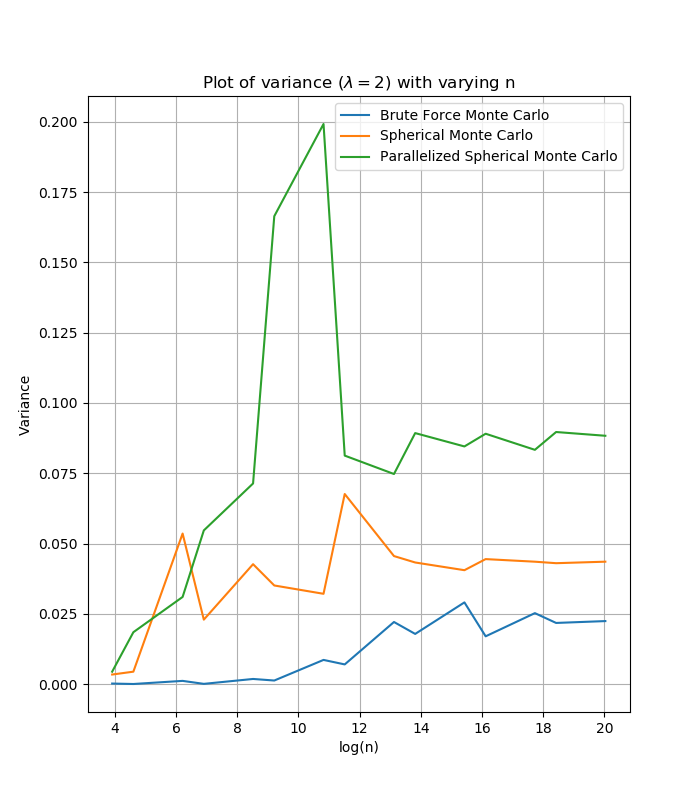
\includegraphics[width = 11cm]{images/variance-montecarlo.png}
    \caption{The plot of variance as a function of the logarithm of integration points $n$ for brute force Monte Carlo, spherical Monte Carlo, and parallelized spherical Monte Carlo. }
    \label{fig:variancemontecarlopng}
  \end{figure}


  \begin{table}[ht]
    \centering
    \caption{Error and execution time for brute force Monte Carlo, spherical Monte Carlo, and parallelized spherical Monte Carlo when testing different compiler optimalization flags with $\lambda = 2$.}
    \vspace{2mm}
    \label{tab:optimalization-montecarlo}
    \begin{tabular}{|c|c|c|c|c|c|c|c|}
        \hline
        Compiler flag & $n$ & BMC error & SMC error & PSMC error & BMC time & SMC time & PSMC time  \\
        \hline \hline
        none & 500000000 & 6.07925e-05 & 2.59234e-05 & 1.66251e-05 & 415.953 & 448.229 & 208.211 \\
        -O & 500000000 & 0.001144 & 3.8324e-05 & 5.9218e-05 & 140.108 & 170.505 & 75.0108 \\
        -O0 & 500000000 & 9.9830e-05 & 1.5527e-05 & 8.7296e-05 & 368.159 & 429.329 & 197.266 \\
        -O1 & 500000000 & 0.0005797 & 2.9770e-05 & 3.3298e-05 & 206.356 & 231.86 & 113.938 \\
        -O2 & 500000000 & 4.7324e-05 & 4.7423e-05 & 2.5998e-05 & 138.492 & 168.688 & 74.8991 \\
        -O3 & 500000000 & 0.001158 & 0.0001025 & 7.5507e-06 & 141.051 & 160.792 & 71.5184 \\
        \hline
    \end{tabular} \\
    \hspace{0pt}\\
  \end{table}
\fi


%--------------- Discussion ---------------------------------------
\vspace{1cm}

\clearpage
\newpage

\section{Discussion} \label{sec:Discussion}




%---------------Conclusion and perspective---------------------------
\vspace{1cm}

\section{Conclusion and perspective} \label{sec:Conclusion}



%--------------Appendix---------------------------------------------
\vspace{1cm}

\section{Appendix} \label{sec:Appendix}



%\clearpage

%----------------References----------------------------------------

\vspace{1cm}

\section{References} \label{sec:References}

\begin{thebibliography}{}

\bibitem{task}
Morten H. Jensen (2019), \href{https://github.com/CompPhysics/ComputationalPhysics/blob/master/doc/Projects/2019/Project3/pdf/Project3.pdf}{Project 3}, Departement of Physics, University of Oslo, Norway

\bibitem{github}
Erik B. Grammeltvedt, Alexandra Jahr Kolstad, Erlend T. North (2019), \href{https://github.com/Erikbgram/Fys3150}{GitHub}, Students of Departement of Physics, University of Oslo, Norway

\bibitem{lecture_slides}
Morten H. Jensen (2015), \href{https://github.com/CompPhysics/ComputationalPhysics/blob/master/doc/Lectures/lectures2015.pdf}{Lecture slides for FYS3150}, Department of Physics, University of Oslo, Norway

\bibitem{laguerre_polynomial}
Weisstein, Eric W. \href{http://mathworld.wolfram.com/LaguerrePolynomial.html}{"Laguerre Polynomial."}, From MathWorld--A Wolfram Web Resource.


\end{thebibliography}


%----------------Slutten av dokumentet---------------------------------------


%\end{multicols}

\end{document}
